A comparative analysis of termination techniques for DPO graph rewriting systems, drawn from prior work~\cite{plump1995ontermination,plump2018modular,bruggink2014termination,bruggink2015proving,endrullis2024generalized_arxiv_v2,overbeek2024termination_lmcs}, is summarized in Table~\ref{tab:comparison:subgraph_counting}. Our approach successfully proves termination for 14 of these systems. In the remainder of this section, we compare our method with some existing methods in more detail.


{% local group
  \setlength{\tabcolsep}{3pt}
  \renewcommand{\arraystretch}{1}
\begin{table}[H]
   \centering
  \small % Reduce font size
  \caption{Applicability of termination techniques to DPO rewriting examples.
  The symbol \ding{51} indicates termination can be proved by the technique,
  \ding{55} indicates it cannot be proved, and 
  $-$ denotes irrelevance or out-of-scope cases.
        }
 \label{tab:comparison:subgraph_counting}
% \setlength{\tabcolsep}{4pt} % Reduce horizontal padding
   \begin{NiceTabular}{ccccccccc}[vlines] % <-- 9 columns now (was 7)
    \Hline
                % \diagbox{\enskip \textbf{Examples}}{\textbf{Techniques}} 
    \Block{1-2}{\diagbox{\enskip \textbf{Examples}}{\textbf{Techniques}}} & 
    &
    \RowStyle{\rotate}
     \makecell{Forward closure \cite{plump1995ontermination}} % NEW column #1
    & \RowStyle{\rotate}
     \makecell{Modular criterion \cite{plump2018modular}} % NEW column #2
    & \RowStyle{\rotate}
     \makecell{Type graph \cite{bruggink2014termination}}  
    & \RowStyle{\rotate}
     \makecell{Type graph \cite{bruggink2015proving}} 
    & \RowStyle{\rotate}
     \makecell{Type graph \cite{endrullis2024generalized_arxiv_v2}} 
    & \RowStyle{\rotate}
     \makecell{Subgraph 
            counting \cite{overbeek2024termination_lmcs}} 
    & \RowStyle{\rotate}
     \makecell{Morphism
                Counting 
                \\(Chapter~\ref{chap:subgraph_counting})} \\
    \Hline
    \Hline
% ok examples
Chapter~\ref{chap:subgraph_counting} 
&Example~\ref{subgraph_counting:ex_contrib_variant}
  & \ding{51} & \ding{55} & \ding{55} & \ding{55} & \ding{55} & \ding{55} & \ding{51} \\ \Hline
  
\cite{plump1995ontermination} &
\hyperref[ex:overbeek_5d8_plump1995_3d8_plump2018_3_overbeek_5d8]{Example 3.8}
             & \ding{51} & -- & -- & -- & -- &
          --
             & \ding{51}\\ 
\hline

\Block{2-1}{\cite{plump2018modular}} & \hyperref[ex:overbeek_5d8_plump1995_3d8_plump2018_3_overbeek_5d8]{Example 3} 
          & -- & \ding{51} &  -- & -- & -- & 
          --
          & \ding{51}\\ 

\Hline

%~\cite{plump2018modular} 
& Example 5 &  -- &  \ding{51} &   -- & -- & -- &  
            --
          & \ding{51}\\  
\Hline

\cite{bruggink2014termination} & \hyperref[{subgraph_counting:ex:termination:bruggink14_ex4_and6}]{Examples 4 and 6}  
  & -- & -- & \ding{51} & -- & -- & 
            --
          & \ding{51} \\ \Hline

\Block{2-1}{\cite{bruggink2015proving}} & \hyperref[subgraph_counting:ex:termination:bruggink15_ex2]{Example 2}  
  & -- & -- & -- & \ding{51} & -- & 
  -- &  \ding{51}\\ \Hline
  
%~\cite{bruggink2015proving}
 & \hyperref[subgraph_counting:ex:bruggink2015_ex4]{Example 4} 
  & -- & -- & -- & \ding{51} & -- & 
  --& \ding{51} \\ \Hline


% ----- from endrullis2024generalized_arxiv_v2 -----
\Block{3-1}{\cite{endrullis2024generalized_arxiv_v2}} & \hyperref[ex:endrullis2024_6d2]{Example 6.2}  
  & -- & -- & -- & -- & \ding{51} & -- & \ding{51}\\ \Hline

%~\cite{endrullis2024generalized_arxiv_v2}
 & \hyperref[ex_endrullis_6d3_endrullis_5d8]{Example 6.3}
  & -- & -- & -- & -- & \ding{51} &% \ding{55} 
  \ding{55} & \ding{51}\\ \Hline

%~\cite{endrullis2024generalized_arxiv_v2} 
& \hyperref[ex:overbeek_5d8_plump1995_3d8_plump2018_3_overbeek_5d8]{Example D.1}
  & -- & -- & -- & -- & \ding{51} & -- & \ding{51}\\ \Hline

  \Block{4-1}{\cite{overbeek2024termination_lmcs}} & \hyperref[ex:overbeek_5d3]{Example 5.3}
  & -- & -- & -- & -- & -- & \ding{51} & \ding{51}\\ \Hline

%~\cite{overbeek2024termination_lmcs} \hyperref[ex:overbeek_5d3]{Example 5.3 monic matches}
%     & -- & -- & -- & -- & -- & \ding{51} & \ding{51}\\ \Hline
%~\cite{overbeek2024termination_lmcs} 
& \hyperref[ex:overbeek_5d5]{Example 5.5} 
  & -- & -- & -- & -- & -- & \ding{51} & \ding{51}\\ \Hline

%~\cite{overbeek2024termination_lmcs} 
& \hyperref[ex:overbeek_5d6]{Example 5.6}
  & -- & -- & -- & -- & -- & \ding{51} & \ding{51} \\ \Hline

%~\cite{overbeek2024termination_lmcs} \hyperref[ex:overbeek_5d6]{Example 5.6 bis}
%     & -- & -- & -- & -- & -- & \ding{51} & -- \\ \Hline


%~\cite{overbeek2024termination_lmcs}  
& \hyperref[ex:overbeek_5d8_plump1995_3d8_plump2018_3_overbeek_5d8]{Example 5.8}
  & -- & -- & -- & -- & -- & \ding{51} & \ding{51}\\ \Hline

      % not supported examples  
     ~\cite{plump2018modular} &  \hyperref[ex:plump2018_ex6_endrullis_d4]{Example 6} &  -- & \ding{51} & -- & -- & -- & 
      --
          & -- \\
      \Hline

\Block{3-1}{\cite{endrullis2024generalized_arxiv_v2}}
 & Example 6.4  
      & -- & -- & -- & -- & \ding{51} & -- & -- \\ \Hline

%  ~\cite{endrullis2024generalized_arxiv_v2}
  &  Example 6.5  
      & -- & -- & -- & -- &  \ding{51} & -- & -- \\ \Hline

    %  ~\cite{endrullis2024generalized_arxiv_v2}
       &\hyperref[ex:plump2018_ex6_endrullis_d4]{Example D.4} 
      & -- & -- & -- & -- & \ding{51} & -- & --\\ \Hline

   % ----- from overbeek2024termination_lmcs -----
   \Block{3-1}{\cite{overbeek2024termination_lmcs}} 
      & \hyperref[ex:overbeek:5d2:limitation]{Example 5.2}
      & -- & -- & -- & -- & -- & \ding{51} & -- \\ \Hline

    %  ~\cite{overbeek2024termination_lmcs} 
      & Example 5.7 
      & -- & -- & -- & -- & -- & \ding{51} & -- \\ \Hline
      
%  ~\cite{overbeek2024termination_lmcs} 
  & Example 5.9 
      & -- & -- & -- & -- & -- & \ding{51} & --\\ \Hline
 

    % not ok examples
   ~\cite{plump1995ontermination} & \hyperref[ex:plump95_4d1]{Example 4.1} & \ding{51} & -- & -- & -- & -- & 
              \ding{51}
              
              & \ding{55}\\ 
   \Hline
  ~\cite{plump2018modular} & \hyperref[ex:plump_ex4]{Example 4} &  -- &  \ding{51} &  -- & -- & -- & 
               --
               & \ding{55}\\ 
   \Hline

   \Block{3-1}{\cite{bruggink2014termination}} & Example 1 
   & -- & -- & \ding{51} & -- & -- & 
                 --
               &  \ding{55}\\ 
   \Hline

%   ~\cite{bruggink2014termination} 
   & Routing Protocol
       & -- & -- & \ding{51} & -- & -- & 
           --
           &  \ding{55}\\  
           \Hline
% \Block{2-1}{\cite{bruggink2014termination}}
 & \hyperref[ex:plump_ex4]{Example 5}
   & -- & -- & \ding{51} & -- & -- & -- &  \ding{55}\\ 
\Hline

\Block{2-1}{\cite{bruggink2015proving}} & \hyperref[ex:bruggink2015_ex5]{Example 5}
   & -- & -- & -- & \ding{51} & -- &  
   -- &  \ding{55}\\
   \Hline

%   ~\cite{bruggink2015proving} 
   & \hyperref[ex:bruggink2015_ex6_endrullis2024_d2]{Example 6} 
   & -- & -- & -- & \ding{51} & -- &  
   --&  \ding{55}\\  
   \Hline

   \Block{2-1}{\cite{endrullis2024generalized_arxiv_v2}} & \hyperref[ex:bruggink2015_ex6_endrullis2024_d2]{Example D.2} 
   & -- & -- & -- & -- & \ding{51} & -- & \ding{55}\\ 
   \Hline

%   ~\cite{endrullis2024generalized_arxiv_v2}
   & \hyperref[ex:endrullis:d3:limitation]{Example D.3}
   & -- & -- & -- & -- & \ding{51} & \ding{55} & \ding{55}\\ \Hline

  \end{NiceTabular}
  % \vspace{2mm}
  % \caption{Applicability of termination techniques to DPO rewriting examples.
  %  The symbol \ding{51} indicates termination can be proved by the technique,
  %  \ding{55} indicates it cannot be proved, and 
  %  $-$ denotes irrelevance or out-of-scope cases.
  %        }
  % \label{tab:comparison}
  \end{table}
} 


The subgraph-counting method by Overbeek and Endrullis~\cite{overbeek2024termination_lmcs} is designed for the PBPO+~\cite{overbeek2023graph, overbeek2023apbpotutorial}\textemdash{}a rewriting formalism capable of simulating left-injective DPO rewriting.
%  It can prove termination for systems like~\cite[Examples 5.2, 5.7, 5.9]{overbeek2024termination_lmcs} and~\cite[Example 6]{plump2018modular}, which lie beyond the scope of our technique. 
 Additionally, this method can be applied for many categories. 

It is very closely related to our work in the setting where they are both defined. Both methods weigh objects by summing weighted morphisms targeting them, and, for both methods, the key challenge lies in estimating weights for morphisms whose images partially overlap with the rewriting context, because morphisms fully embedded in the context are shared between host and resulting graphs, while those entirely within left- or right-hand-side graphs are trivial to quantify.  

The two methods employ distinct strategies to overcome this challenge. The subgraph counting method relies on type-morphisms (see~\cite[page 9, remark 4.11, Lemma 4.23]{overbeek2024termination_lmcs}), whereas our approach requires injective mappings from (i) subgraph occurrences partially overlapping the rewriting context in the result graph to (ii) those in the host graph.

Both approaches have limitations and strengths. Endrullis and Overbeek's approach suffers from discrete interface\textemdash{}interface graph with no edges, as mentioned in~\cite[Example 5.5]{overbeek2024termination_lmcs}. For instance, it proves termination of Example~\ref{ex:overbeek_5d5}:
\begin{center}
      \resizebox{0.95\textwidth}{!}{
          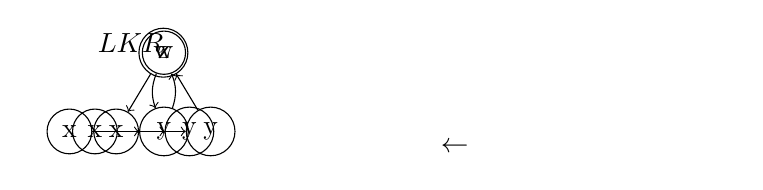
\begin{tikzpicture}
              \graphbox{$L$}{0mm}{0mm}{35mm}{25mm}{2mm}{-8mm}{
                  \coordinate (delta) at (0,-18mm);
                  \node[draw,circle] (x) at (-6mm,-10mm) {x};
                  \node[draw,circle] (y) at (6mm,-10mm) {y};
                  \node[draw,circle]  (z) at (6mm,0mm) {z};
                  \draw[->]  (x) to (y);
                  \draw[->] (y) to[bend right=20] (z);
                  \draw[->]  (z) to[bend right=20] (y);
              }
              \graphbox{$K$}{40mm}{0mm}{35mm}{25mm}{2mm}{-8mm}{
                  \node[draw,circle]  (x) at (-6mm,-10mm) {x};
                  \node[draw,circle]  (y) at (6mm,-10mm) {y};
                  \draw[->] (x) to (y);
              }
              \graphbox{$R$}{80mm}{0mm}{35mm}{25mm}{2mm}{-8mm}{
                  \node[draw,circle]  (x) at (-6mm,-10mm) {x};
                      \node[draw,circle]  (y) at (6mm,-10mm) {y};
                      \node[draw,circle]  (z) at (0mm,0mm) {w};
                      \draw[->]  (x) to (y);
                      \draw[->]  (y) to [bend left=0] (z);
                      \draw[->]  (z) to [bend left=0] (x);
              }
              \node () at (37mm,-12mm) {$\leftarrow$};
              \node () at (78mm,-12mm) {$\rightarrow$};
          \end{tikzpicture}
      }
  \end{center}
   but fails for Example~\ref{ex_endrullis_6d3_endrullis_5d8}:
   \begin{center}
          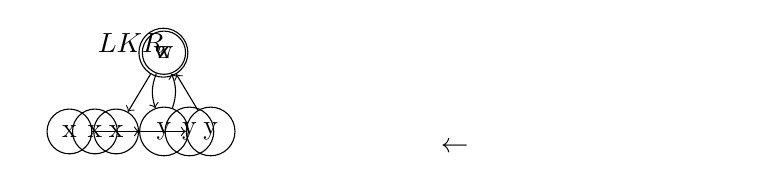
\begin{tikzpicture}
              \graphbox{$L$}{0mm}{0mm}{35mm}{25mm}{2mm}{-8mm}{
                  \coordinate (delta) at (0,-18mm);
                  \node[draw,circle] (x) at (-6mm,-10mm) {x};
                  \node[draw,circle] (y) at (6mm,-10mm) {y};
                  \node[draw,circle]  (z) at (6mm,0mm) {z};
                  \draw[->]  (x) to (y);
                  \draw[->] (y) to[bend right=20] (z);
                  \draw[->]  (z) to[bend right=20] (y);
              }
              \graphbox{$K$}{40mm}{0mm}{35mm}{25mm}{2mm}{-8mm}{
                  \node[draw,circle]  (x) at (-6mm,-10mm) {x};
                  \node[draw,circle]  (y) at (6mm,-10mm) {y};
              }
              \graphbox{$R$}{80mm}{0mm}{35mm}{25mm}{2mm}{-8mm}{
                  \node[draw,circle]  (x) at (-6mm,-10mm) {x};
                      \node[draw,circle]  (y) at (6mm,-10mm) {y};
                      \node[draw,circle]  (z) at (0mm,0mm) {w};
                      \draw[->]  (x) to (y);
                      \draw[->]  (y) to [bend left=0] (z);
                      \draw[->]  (z) to [bend left=0] (x);
              }
              \node () at (37mm,-12mm) {$\leftarrow$};
              \node () at (78mm,-12mm) {$\rightarrow$};
          \end{tikzpicture}
  \end{center}
% ~\cite[Example 6.3]{endrullis2024generalized_arxiv_v2}
while the rules differ only by an edge in the interface graph.
Similarly, it fails to prove termination for Example~\ref{subgraph_counting:ex_contrib_variant}:
 \begin{center}
            \begin{tikzpicture}[scale=0.9]
                \graphbox{$L$}{0mm}{0mm}{35mm}{35mm}{2mm}{-5mm}{
                    \coordinate (delta) at (0,-18mm);
                    \node[draw,circle] (l1) at ($(delta)+(-1,1.5)$) {$1$};
                    \node[draw,circle] (l2) at ($(delta)+(1,1.5)$) {$2$};
                    \node[draw,circle] (l3) at ($(delta)+(0,0)$) {3};
                    \draw[->] (l1) -- (l3) node[midway,left] {$s$};
                    \draw[->] (l2) -- (l3) node[midway,right] {$s$};
                    \draw[->] (l3) edge [loop below] node {$0$} (l3);
                }
                \graphbox{$K$}{40mm}{0mm}{35mm}{35mm}{2mm}{-5mm}{
                    \coordinate (delta) at (0,-18mm);
                    \coordinate (interfaceorigin) at ($(delta) +(5,0)$);
                    \node[draw,circle] (r1) at ($(delta) +(-1,1.5)$) {$1$};
                    \node[draw,circle] (r2) at ($(delta) +(0.5,1.5)$) {$2$};
                    \node[draw,circle] (r3) at ($(delta)+(0,0)$) {3};
                    % \draw[->] (r1) -- (r3) node[midway,left] {$s$};
                    % \draw[->] (r3) edge [loop below] node {$0$} (r3);
                }
                \graphbox{$R$}{80mm}{0mm}{50mm}{35mm}{2mm}{-5mm}{
                    \coordinate (delta) at (-10mm,-18mm);
                    \node[draw,circle] (r1) at ($(delta)+(-1,1.5)$) {$1$};
                    \node[draw,circle] (r2) at ($(delta)+(0.5,1.5)$) {$2$};
                    \node[draw,circle] (r3) at ($(delta)+(0,0)$) {3};
                    \node[draw,circle] (r4) at ($(delta)+(1,0)$) {4};
                    \draw[->] (r1) -- (r3) node[midway,left] {$s$};
                    \draw[->] (r2) -- (r4) node[midway,right] {$s$};
                    \draw[->] (r4) edge [loop below] node {$0$} (r4);
                    \draw[->] (r3) edge [loop below] node {$0$} (r3);
                    \node[draw,circle] (r5) at ($(r2)+(1.5,0)$) {};
                    \draw[->] (r5) edge [loop below] node {$0$} (r5);
                    \draw[->] (r5) edge [loop right] node {$0$} (r5);
                    \draw[->] (r5) edge [loop left] node {$0$} (r5);
                }
                \node () at (38mm,-18mm) {$\leftarrow$};
                \node () at (77mm,-18mm) {$\rightarrow$};
            \end{tikzpicture}
          \end{center}
      but if an edge labeled by ``s'' from node $1$ to node $3$ is added to the interface graph, then it succeeds. Our approach, however, can handle all the aforementioned cases. Nevertheless, their method can address the system in Example~\ref{ex:plump95_4d1}:
        \begin{center}
    $\rho'\mathop{=}$\scalebox{0.9} { {
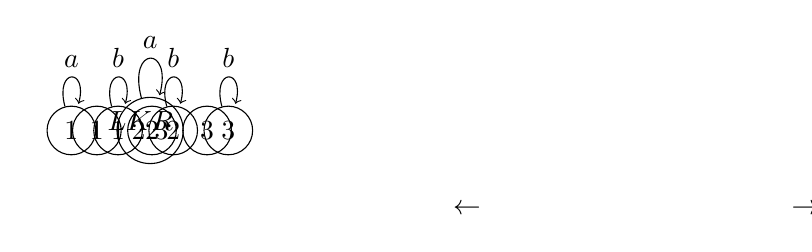
\begin{tikzpicture}[baseline=-10mm]
    \graphbox{$L$}{0mm}{0mm}{38mm}{20mm}{2mm}{-13mm}{
      \node [draw, circle] (x) at (-7mm,0mm) {1};
      \node [draw, circle] (y) at (3mm,0mm) {2 3};
      \draw[->] (x) edge[loop above] node  {$a$} (x);
      \draw[->] (y) edge [loop above] node {$a$} (y);
    }
    \graphbox{$K$}{42mm}{-0mm}{38mm}{20mm}{0mm}{-10mm}{
        \node [draw, circle] (x) at (-7mm,0mm) {1};
        \node [draw, circle] (y) at (0mm,0mm) {2};
        \node [draw, circle] (z) at (7mm,0mm) {3};    
    }
    \begin{scope}[opacity=1]        
    \graphbox{$R$}{85mm}{-0mm}{38mm}{20mm}{2mm}{-13mm}{
      \node [draw, circle] (x) at (-7mm,0mm) {1};
      \node [draw, circle] (y) at (0mm,0mm) {2};
      \node [draw, circle] (z) at (7mm,0mm) {3};
      \draw[->] (x) edge[loop above] node  {$b$} (x);
      \draw[->] (y) edge[loop above] node  {$b$} (y);
      \draw[->] (z) edge[loop above] node  {$b$} (z);
    }
    \end{scope}
    \node () at (40mm,-10mm) {$\leftarrow$};
    \node () at (83mm,-10mm) {$\rightarrow$};
\end{tikzpicture}
}

}
    % \caption{}
    % \label{fig:subgraph_counting:ex_overbeek_5d6_bis}
  \end{center} 
% (~\cite[\hyperref[ex:plump95_4d1]{Example 4.1}]{plump1995ontermination}) 
which remains beyond the scope of our technique. Finally, both approaches cannot handle Example~\ref{ex:endrullis:d3:limitation} (see~\cite[Remark 6.2]{overbeek2024termination_lmcs}).
% ,
% ~\cite[Example D.3]{endrullis2024generalized_arxiv_v2} (see~\cite[Remark 6.2]{overbeek2024termination_lmcs} and Example~\ref{ex:endrullis:d3:limitation}).
% The type graph method, which weighs an object by summing the weights of morphisms from the object to a type graph, was initially introduced by Zantema, K{\"o}nig and Bruggink~\cite{zantema2014termination} for cycle-rewriting systems. 
% This method has since been generalized to edge-labeled multigraphs by Bruggink et al.~\cite{bruggink2014termination} for DPO rewriting with monic matches and injective rules, later extended to DPO rewriting in general by Bruggink et al.~\cite{bruggink2015proving}, and further adapted to more categories and different DPO variants by Endrullis et al.~\cite{endrullis2024generalized_arxiv_v2}. 
% These methods are not directly comparable with our technique in general.

The type graph method is also related to our approach, as both methods involve counting morphisms. However, they differ in direction: the type graph method counts morphisms from the object to a fixed type graph, while our method counts morphisms from a fixed pattern graph to the object.
Concerning their applicability, neither method strictly subsumes the other.
On the one hand, the termination of Example~\ref{subgraph_counting:ex_contrib_variant}, shown below, can be proved by our method but not by the type graph methods due to the existence of a surjection from the output graph to the input graph as explained in~\cite[Example D.4]{endrullis2024generalized_arxiv_v2}.
\begin{center}
            \begin{tikzpicture}[scale=0.9]
                \graphbox{$L$}{0mm}{0mm}{35mm}{35mm}{2mm}{-5mm}{
                    \coordinate (delta) at (0,-18mm);
                    \node[draw,circle] (l1) at ($(delta)+(-1,1.5)$) {$1$};
                    \node[draw,circle] (l2) at ($(delta)+(1,1.5)$) {$2$};
                    \node[draw,circle] (l3) at ($(delta)+(0,0)$) {3};
                    \draw[->] (l1) -- (l3) node[midway,left] {$s$};
                    \draw[->] (l2) -- (l3) node[midway,right] {$s$};
                    \draw[->] (l3) edge [loop below] node {$0$} (l3);
                }
                \graphbox{$K$}{40mm}{0mm}{35mm}{35mm}{2mm}{-5mm}{
                    \coordinate (delta) at (0,-18mm);
                    \coordinate (interfaceorigin) at ($(delta) +(5,0)$);
                    \node[draw,circle] (r1) at ($(delta) +(-1,1.5)$) {$1$};
                    \node[draw,circle] (r2) at ($(delta) +(0.5,1.5)$) {$2$};
                    \node[draw,circle] (r3) at ($(delta)+(0,0)$) {3};
                    % \draw[->] (r1) -- (r3) node[midway,left] {$s$};
                    % \draw[->] (r3) edge [loop below] node {$0$} (r3);
                }
                \graphbox{$R$}{80mm}{0mm}{50mm}{35mm}{2mm}{-5mm}{
                    \coordinate (delta) at (-10mm,-18mm);
                    \node[draw,circle] (r1) at ($(delta)+(-1,1.5)$) {$1$};
                    \node[draw,circle] (r2) at ($(delta)+(0.5,1.5)$) {$2$};
                    \node[draw,circle] (r3) at ($(delta)+(0,0)$) {3};
                    \node[draw,circle] (r4) at ($(delta)+(1,0)$) {4};
                    \draw[->] (r1) -- (r3) node[midway,left] {$s$};
                    \draw[->] (r2) -- (r4) node[midway,right] {$s$};
                    \draw[->] (r4) edge [loop below] node {$0$} (r4);
                    \draw[->] (r3) edge [loop below] node {$0$} (r3);
                    \node[draw,circle] (r5) at ($(r2)+(1.5,0)$) {};
                    \draw[->] (r5) edge [loop below] node {$0$} (r5);
                    \draw[->] (r5) edge [loop right] node {$0$} (r5);
                    \draw[->] (r5) edge [loop left] node {$0$} (r5);
                }
                \node () at (38mm,-18mm) {$\leftarrow$};
                \node () at (77mm,-18mm) {$\rightarrow$};
            \end{tikzpicture}
          \end{center}
        On the other hand, our method cannot prove the termination of Example~\ref{ex:endrullis:d3:limitation}, shown below, because of the injection from the left-hand side graph $L$ to the right-hand side graph $R$, but the type graph methods can handle it.
    \begin{center}
        \begin{tikzpicture}  
          \graphbox{$L$}{0mm}{-11mm}{32mm}{15mm}{2mm}{-8mm}{  
              \node[draw,circle]  (x) at (-6mm,0mm) {$1$};  
              \node[draw,circle]  (y) at (6mm,0mm) {};  
            }  
            \graphbox{$K$}{36mm}{-11mm}{32mm}{15mm}{2mm}{-8mm}{  
              \node[draw,circle]  (x) at (-6mm,0mm) {$1$};  
            }  
            \graphbox{$R$}{72mm}{-11mm}{32mm}{15mm}{1mm}{-8mm}{  
              \node[draw,circle]  (x) at (-6mm,0mm) {$1$};  
              \node[draw,circle]  (y) at (6mm,0mm) {};  
              \draw[->]  (x) to (y);  
            }    
              \node () at (34mm,-19mm) {$\leftarrow$};
              \node () at (70mm,-19mm) {$\rightarrow$};
      \end{tikzpicture}
    \end{center}
          %  On the other hand, our method cannot prove the termination of~\cite[Example 1, 5 and Ad-hoc Routing Protocol]{bruggink2014termination}, nor~\cite[Example 5, 6]{bruggink2015proving}, nor~\cite[Examples D2 and D3]{endrullis2024generalized_arxiv_v2}.

Plump~\cite{plump1995ontermination} gives a necessary and sufficient termination criterion for left-injective DPO hypergraph rewriting in terms of forward closure. Here, a hypergraph generalizes a graph: its edges (hyperedges) may connect more than two vertices. Deciding whether a system satisfies forward closure is undecidable, since forward closure holds if and only if the rewriting system terminates.
% While this method proves termination of Example~\ref{subgraph_counting:ex_contrib_variant}, our approach succeeds on~\cite[Example 3.8]{plump1995ontermination} but fails in proving termination of~\cite[Example 4.1]{plump1995ontermination}. 

Plump~\cite{plump2018modular} later proposed a modular critical pair-based strategy for left-injective DPO hypergraph rewriting with monic matches.
It decomposes a rewriting system into two subsystems, each of which can be analyzed separately using arbitrary termination techniques, and if both subsystems terminate, then the entire system terminates.
Our method complements this: while modularity reduces global complexity, each subsystem requires individual termination proofs.  
For example, the measure based on the indegree proposed in~\cite{plump2018modular} cannot prove the termination of Example~\ref{subgraph_counting:ex_contrib_variant}, illustrated below, due to the loops on the node 5 in the right-hand side graph $R$. 
\begin{center}
            \begin{tikzpicture}[scale=0.9]
                \graphbox{$L$}{0mm}{0mm}{35mm}{35mm}{2mm}{-5mm}{
                    \coordinate (delta) at (0,-18mm);
                    \node[draw,circle] (l1) at ($(delta)+(-1,1.5)$) {$1$};
                    \node[draw,circle] (l2) at ($(delta)+(1,1.5)$) {$2$};
                    \node[draw,circle] (l3) at ($(delta)+(0,0)$) {3};
                    \draw[->] (l1) -- (l3) node[midway,left] {$s$};
                    \draw[->] (l2) -- (l3) node[midway,right] {$s$};
                    \draw[->] (l3) edge [loop below] node {$0$} (l3);
                }
                \graphbox{$K$}{40mm}{0mm}{35mm}{35mm}{2mm}{-5mm}{
                    \coordinate (delta) at (0,-18mm);
                    \coordinate (interfaceorigin) at ($(delta) +(5,0)$);
                    \node[draw,circle] (r1) at ($(delta) +(-1,1.5)$) {$1$};
                    \node[draw,circle] (r2) at ($(delta) +(0.5,1.5)$) {$2$};
                    \node[draw,circle] (r3) at ($(delta)+(0,0)$) {3};
                    % \draw[->] (r1) -- (r3) node[midway,left] {$s$};
                    % \draw[->] (r3) edge [loop below] node {$0$} (r3);
                }
                \graphbox{$R$}{80mm}{0mm}{50mm}{35mm}{2mm}{-5mm}{
                    \coordinate (delta) at (-10mm,-18mm);
                    \node[draw,circle] (r1) at ($(delta)+(-1,1.5)$) {$1$};
                    \node[draw,circle] (r2) at ($(delta)+(0.5,1.5)$) {$2$};
                    \node[draw,circle] (r3) at ($(delta)+(0,0)$) {$3$};
                    \node[draw,circle] (r4) at ($(delta)+(1,0)$) {$4$};
                    \draw[->] (r1) -- (r3) node[midway,left] {$s$};
                    \draw[->] (r2) -- (r4) node[midway,right] {$s$};
                    \draw[->] (r4) edge [loop below] node {$0$} (r4);
                    \draw[->] (r3) edge [loop below] node {$0$} (r3);
                    \node[draw,circle] (r5) at ($(r2)+(1.5,0)$) {5};
                    \draw[->] (r5) edge [loop below] node {$0$} (r5);
                    \draw[->] (r5) edge [loop right] node {$0$} (r5);
                    \draw[->] (r5) edge [loop left] node {$0$} (r5);
                }
                \node () at (38mm,-18mm) {$\leftarrow$};
                \node () at (77mm,-18mm) {$\rightarrow$};
            \end{tikzpicture}
          \end{center}
Specifically, consider the following rewriting step with the rule:
\begin{center}
            \begin{tikzpicture}[scale=0.9]
                \graphbox{$G$}{0mm}{0mm}{35mm}{35mm}{2mm}{-5mm}{
                    \coordinate (delta) at (0,-18mm);
                    \node[draw,circle] (l1) at ($(delta)+(-1,1.5)$) {$1$};
                    \node[draw,circle] (l2) at ($(delta)+(1,1.5)$) {$2$};
                    \node[draw,circle] (l3) at ($(delta)+(0,0)$) {3};
                    \draw[->] (l1) -- (l3) node[midway,left] {$s$};
                    \draw[->] (l2) -- (l3) node[midway,right] {$s$};
                    \draw[->] (l3) edge [loop below] node {$0$} (l3);
                }
                \graphbox{$H$}{40mm}{0mm}{50mm}{35mm}{2mm}{-5mm}{
                    \coordinate (delta) at (-10mm,-18mm);
                    \node[draw,circle] (r1) at ($(delta)+(-1,1.5)$) {$1$};
                    \node[draw,circle] (r2) at ($(delta)+(0.5,1.5)$) {$2$};
                    \node[draw,circle] (r3) at ($(delta)+(0,0)$) {$3$};
                    \node[draw,circle] (r4) at ($(delta)+(1,0)$) {$4$};
                    \draw[->] (r1) -- (r3) node[midway,left] {$s$};
                    \draw[->] (r2) -- (r4) node[midway,right] {$s$};
                    \draw[->] (r4) edge [loop below] node {$0$} (r4);
                    \draw[->] (r3) edge [loop below] node {$0$} (r3);
                    \node[draw,circle] (r5) at ($(r2)+(1.5,0)$) {5};
                    \draw[->] (r5) edge [loop below] node {$0$} (r5);
                    \draw[->] (r5) edge [loop right] node {$0$} (r5);
                    \draw[->] (r5) edge [loop left] node {$0$} (r5);
                }
                \node () at (38mm,-18mm) {$\Rightarrow$};
            \end{tikzpicture}
          \end{center}
For all $k \mathop{\in} \mathbb{N}$, the weight of the host graph $G$\textemdash{}defined as the sum of node indegrees raised to the power of $k$\textemdash{}is $0^k + 0^k + 3^k = 3^k$, while the weight of the result graph $H$ is $0^k + 0^k + 2^k + 2^k + 3^k = 2^k + 2^k + 3^k$. Since $3^k < 2^k + 2^k + 3^k$, the weight does not decrease. However, our method succeeds (see Example~\ref{subgraph_counting:ex_contrib_variant}).
% Additionally, our method proves termination of~\cite[Examples 1 and 5]{plump2018modular} but not~\cite[Example 4]{plump2018modular}, and non-injective rules (e.g.,~\cite[Example 6]{plump2018modular}) fall outside our scope.

In~\cite{levendovszky2007termination}, a termination criterion for DPO rewriting with monic matches, injective rules and negative application conditions on finite typed attributed graphs is proposed. It is based on the fact that if the application of every infinite sequence of rules requires the initial graph to be infinite, then the system terminates. This technique is theoretically very interesting, but it is hard to check the termination condition automatically.

Bottoni et al.~\cite{bottoni2005termination} present a termination criterion for DPO and SPO rewriting on high-level replacement units. The high-level replacement units that they consider are rewriting systems with very restrictive external control mechanisms. \todo{todo to do: xu : jamais introduit} The method relies on a measuring function satisfying a very strong constraint, and the instance of such a measuring function proposed is node and edge counting, which is subsumed by our method in the setting of DPO rewriting with injective rules.

Bottoni et al.~\cite{bottoni2010atermination} present a criterion for termination of DPO rewriting with monic matches, injective rules and negative application conditions, based on the construction of a labeled transition system,
whose states represent overlaps between the negative application condition and the right-hand side that can give rise to cycles.

Levendovszky et al.~\cite{levendovszky2007termination} propose a termination criterion for DPO rewriting (monic matches, injective rules, negative application conditions), though automated verification is hard as explained in~\cite[\textsection 6]{levendovszky2007termination}. 





